\chapter{Preventivo}
Di seguito viene riportato il preventivo per il progetto MegAlexa; esso si divide,per ogni periodo,in:
\begin{itemize}
	\item \textbf{Prospetto orario:} presenta la distribuzione oraria e la suddivisione nei ruoli per ogni membro del gruppo ZeroSeven;
	\item \textbf{Prospetto economico:}presenta le ore di impegno calcolate per i ruoli coinvolti ed il rispettivo costo;
\end{itemize}
La suddivisione oraria viene svolta avendo come riferimento le seguenti regole:
\begin{itemize}
	\item Ogni membro del gruppo deve coprire ogni ruolo almeno una volta durante il ciclo di sviluppo del prodotto;
	\item Il totale delle ore di lavoro dovrà essere equamente distribuito tra i membri;
	\item Non ci devono essere conflitti di interesse in cui un Verificatore debba controllare il proprio lavoro.
\end{itemize}
Le sigle utilizzate per i vari ruoli saranno:
\begin{itemize}
	\item \textbf{Re:} Responsabile di Progetto;
	\item \textbf{Am:} Amministratore;
	\item \textbf{An:} Analista;
	\item \textbf{Pt:} Progettista;
	\item \textbf{Pr:} Programmatore;
	\item \textbf{Ve:} Verificatore;
\end{itemize}

Per il preventivo si tiene conto che i periodi di Analisi dei Requisiti e di Analisi dei Requisiti di Dettaglio sono considerati di investimento del gruppo e  non a carico dei committente, per cui  le ore di impegno svolte durante questi non saranno conteggiate nelle ore totali da retribuire.

\newpage
\section{Analisi  dei Requisiti}
\subsection{Prospetto orario}
Il prospetto orario per il periodo di Analisi dei Requisiti è illustrato nella seguente tabella:
\begin{table}[!ht]
	\begin{center}  	
		\begin{tabular}{c}
			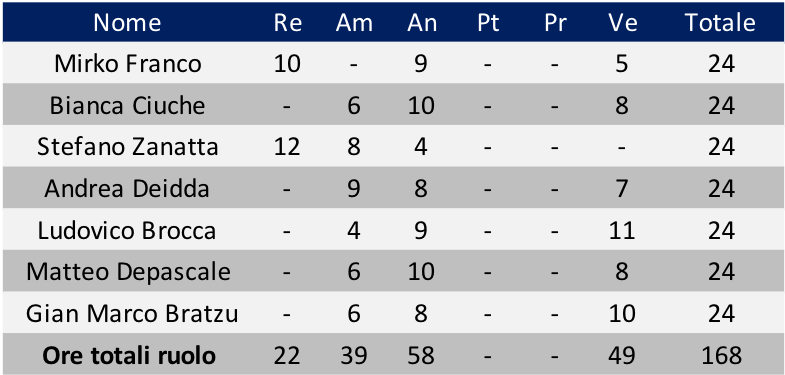
\includegraphics{images/tabellaProspettoOrario.png}
		\end{tabular}
		\caption{Prospetto Orario nel periodo di Analisi dei Requisiti}
	\end{center}
\end{table}

Il seguente grafico rappresenta la suddivisione oraria dei ruoli all'interno del gruppo:
\begin{figure}[!ht]
	\begin{center}
		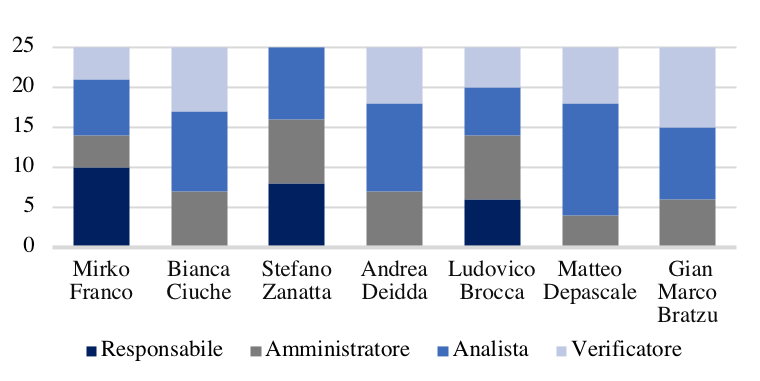
\includegraphics{images/grafoProspettoOrario.png}
		\caption{Grafico prospetto orario nel periodo di Analisi dei Requisiti }
	\end{center}
\end{figure}

\subsection{Prospetto Economico}
Il prospetto economico per il periodo di Analisi dei Requisiti è illustrato nella seguente tabella.
Le spese per questa attività non sono a carico del committente.

\begin{table}[!ht]
	\begin{center}
		\begin{tabular}{c}
			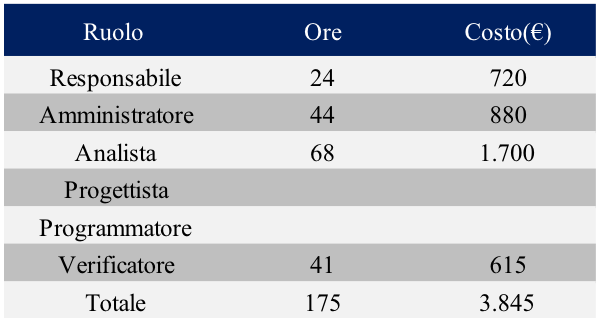
\includegraphics{images/tabellaProspettoEconomico.png}
		\end{tabular}
		\caption{Prospetto Economico nel periodo di Analisi dei Requisiti}
	\end{center}
\end{table}
La raffigurazione grafica del peso di ogni ruolo sul costo totale è così rappresentata:
\begin{figure}[!ht]
	\centering
	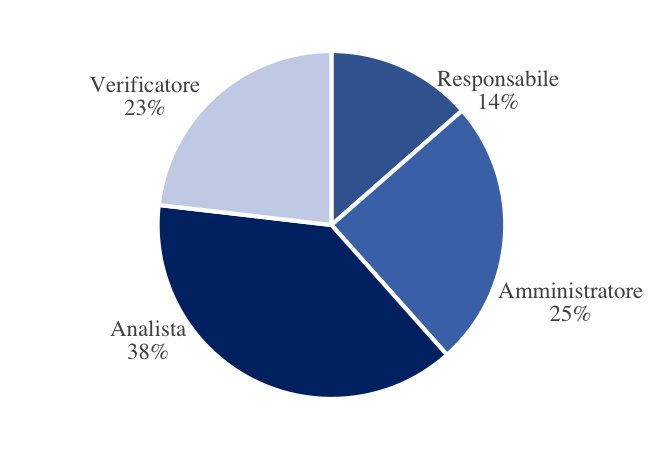
\includegraphics{images/grafoProspettoEconomico.png}
	\caption{Grafico prospetto economico nel periodo di Analisi dei Requisiti }
\end{figure}

\newpage
\section{Analisi dei Requisiti di Dettaglio}
\subsection{Prospetto Orario}
Il prospetto orario per il periodo di Analisi dei Requisiti di Dettaglio è illustrato nella seguente tabella:

\begin{table}[!ht]
	\begin{center}
		\begin{tabular}{c}
			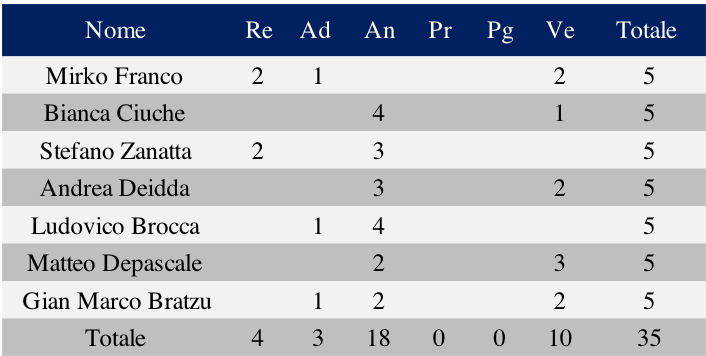
\includegraphics[scale=0.90]{images/tabellaProspettoOrarioDett.png}
		\end{tabular}
		\caption{Prospetto Orario nel periodo di Analisi dei Requisiti di Dettaglio}
	\end{center}
\end{table}
Il seguente grafico rapresenta la suddivisione oraria dei ruoli all'interno del gruppo:
\begin{figure}[!ht]
	\begin{center}
		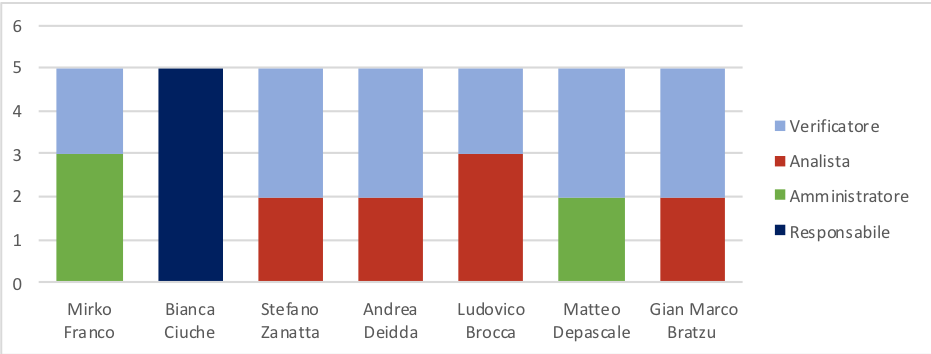
\includegraphics{images/grafoProspettoOrarioDett.png}
		\caption{Grafico prospetto orario nel periodo di Analisi dei Requisiti in Dettaglio}
	\end{center}
\end{figure}
\newpage
\subsection{Prospetto economico}
Il prospetto economico per il periodo di Analisi dei Requisiti di Dettaglio è illustrato nella seguente tabella.
Le spese per questa attività non sono a carico del committente.

\begin{table}[!ht]
	\begin{center}
		\begin{tabular}{c}
			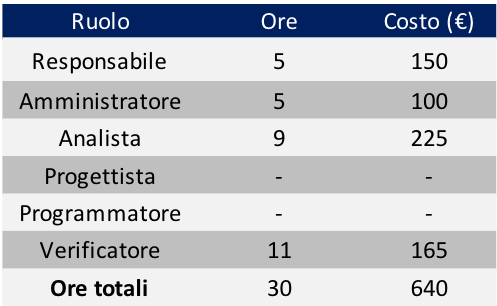
\includegraphics{images/tabellaProspettoEconomicoDett.png}
		\end{tabular}
		\caption{Prospetto Economico nel periodo di Analisi dei Requisiti di Dettaglio}
	\end{center}
\end{table}

La raffigurazione grafica del peso di ogni ruolo sul costo totale è così rappresentata:
\begin{figure}[!ht]
	\begin{center}
		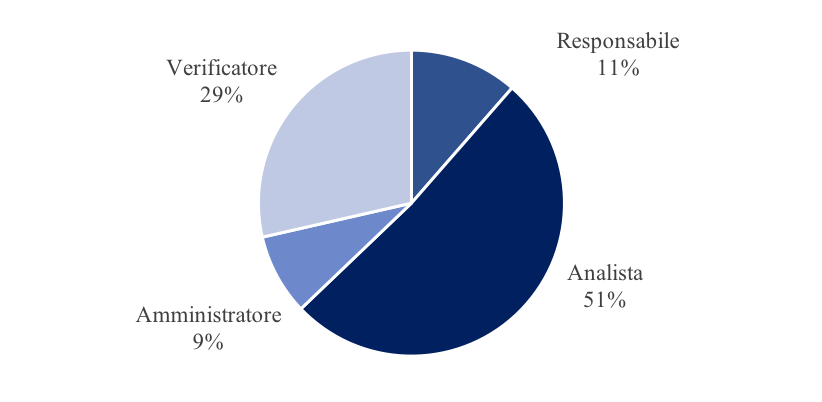
\includegraphics{images/grafoProspettoEconomicoDett.png}
		\caption{Grafico prospetto economico nel periodo di Analisi dei requisiti in dettaglio }
	\end{center}
\end{figure}

\newpage
\section{Progettazione della Base Tecnologica}
\subsection{Prospetto orario}
Il prospetto orario durante il periodo di Progettazione della Base Tecnologica è illustrato nella seguente tabella:

\begin{table}[!ht]
	\begin{center}
		\begin{tabular}{c}
			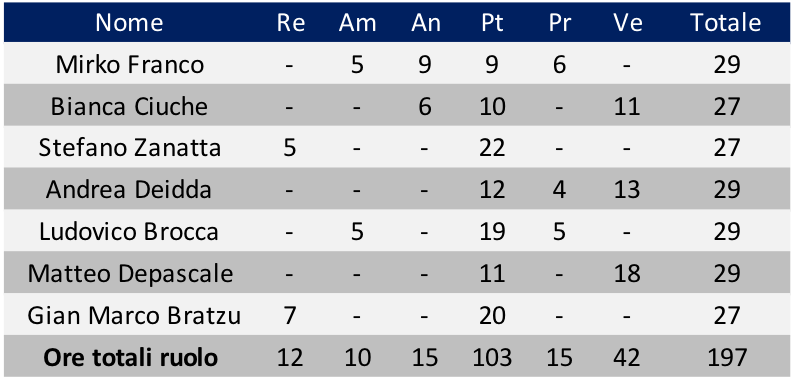
\includegraphics{images/tabellaProgettazioneTecnologica.png}
		\end{tabular}
		\caption{Prospetto Orario nel periodo di Progettazione della Base Tecnologica}
	\end{center}
\end{table}

Il seguente grafico rapresenta la suddivisione oraria dei ruoli all'interno del gruppo:
\begin{figure}[!ht]
	\begin{center}
		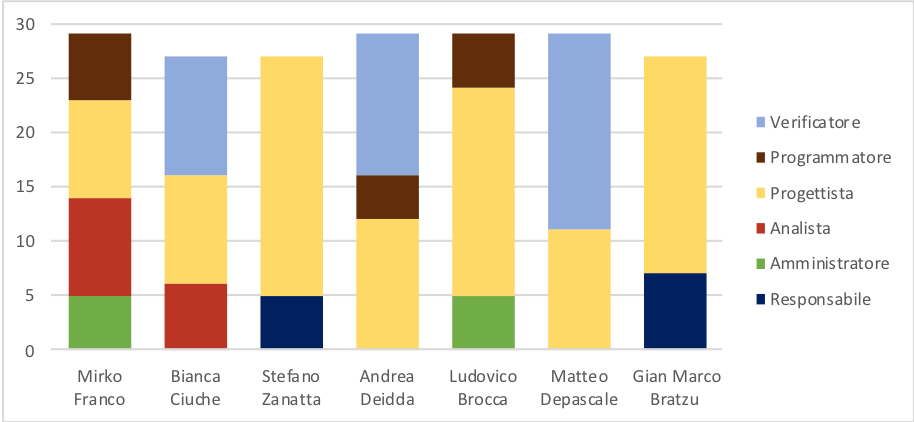
\includegraphics[scale=0.80]{images/grafoProgettazioneTecnologica.png}
		\caption{Grafico prospetto economico nel periodo di Progettazione della Base Tecnologica}
	\end{center}
\end{figure}
\newpage
\subsection{Prospetto economico}
Il prospetto economico per il periodo di Progettazione della Base Tecnologica è illustrato nella seguente tabella:

\begin{table}[!ht]
	\begin{center}
		\begin{tabular}{c}
			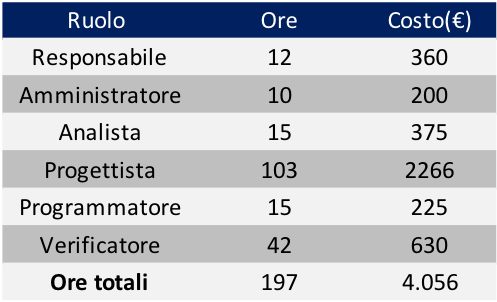
\includegraphics{images/tabellaProgettazioneTecnologicaEuro.png}
		\end{tabular}
		\caption{Prospetto Economico nel periodo di Progettazione della Base Tecnologica}
	\end{center}
\end{table}

La raffigurazione grafica del peso di ogni ruolo sul costo totale è così rappresentata:
\begin{figure}[!ht]
	\begin{center}
		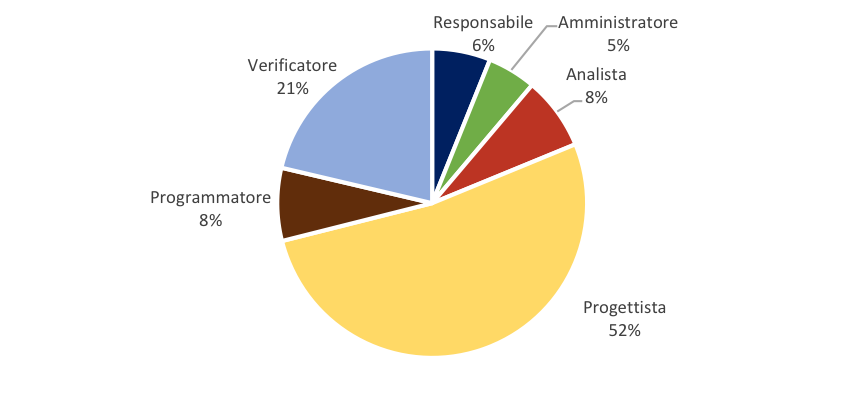
\includegraphics{images/grafoProgettazioneTecnologicaEuro.png}
		\caption{Grafico prospetto orario nel periodo di Analisi dei requisiti in dettaglio}
	\end{center}
\end{figure}
\newpage
\section{Progettazione di Dettaglio e Codifica}
\subsection{Prospetto orario}
Il prospetto orario durante il periodo di Progettazione di Dettaglio e Codifica è illustrato nella seguente tabella:

\begin{table}[!ht]
	\begin{center}
		\begin{tabular}{c}
			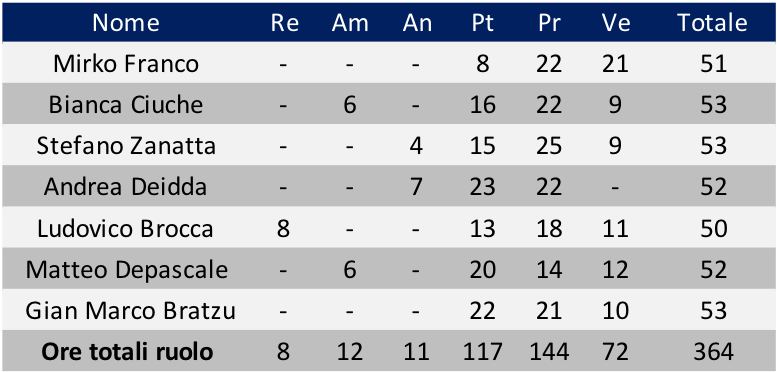
\includegraphics[scale=0.90]{images/tabellaProgettazioneDettaglioCodifica.png}
		\end{tabular}
		\caption{Prospetto orario nel periodo di Progettazione di Dettaglio e Codifica}
	\end{center}
\end{table}

Il seguente grafico mostra una rappresentazione visiva della suddivisione oraria dei ruoli all'interno del gruppo:
\begin{figure}[!ht]
	\begin{center}
		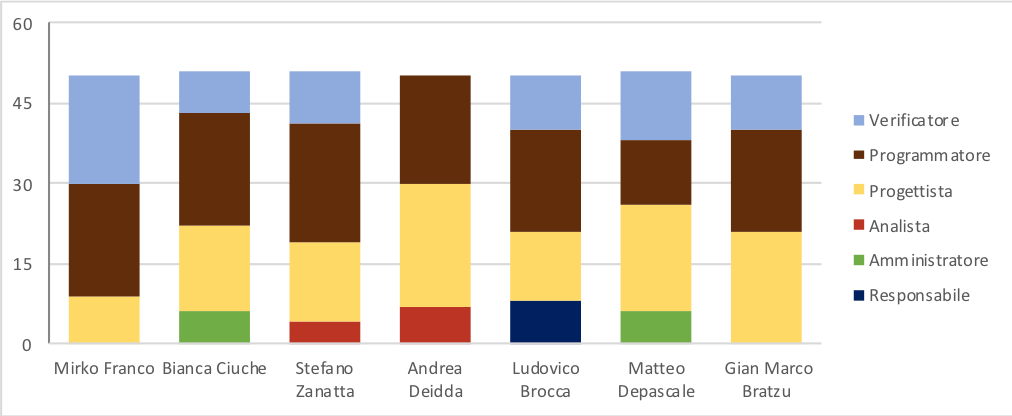
\includegraphics[scale=0.80]{images/grafoProgettazioneDettaglioCodifica.png}
		\caption{Grafico prospetto orario nel periodo di Progettazione di Dettaglio e Codifica}
	\end{center}
\end{figure}

\subsection{Prospetto economico}
Il prospetto economico durante il periodo di Progettazione di Dettaglio e Codifica è illustrato nella seguente tabella:

\begin{table}[!ht]
	\begin{center}
		\begin{tabular}{c}
			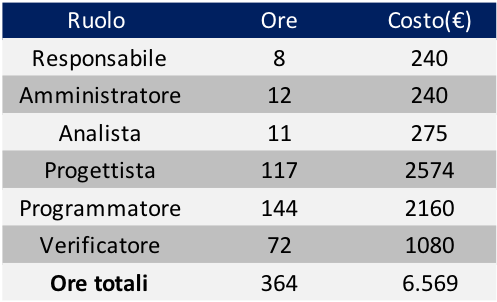
\includegraphics{images/tabellaProgettazioneDettaglioCodificaEuro.png}
		\end{tabular}
		\caption{Prospetto Economico nel periodo di Progettazione di Dettaglio e Codifica}
	\end{center}
\end{table}

\begin{figure}[!ht]
	\begin{center}
		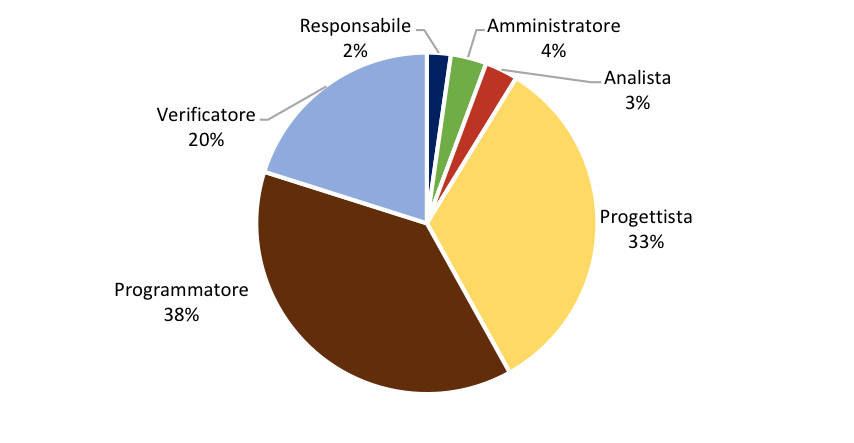
\includegraphics{images/grafoProgettazioneDettaglioCodificaEuro.png}
		\caption{Grafico prospetto economico nel periodo di Progettazione di Dettaglio e Codifica}
	\end{center}
\end{figure}

\newpage
\section{Validazione e Collaudo}
\subsection{Prospetto orario}
Il prospetto orario durante il periodo di Validazione e Collaudo è illustrato nella seguente tabella:

\begin{table}[!ht]
	\begin{center}
		\begin{tabular}{c}
			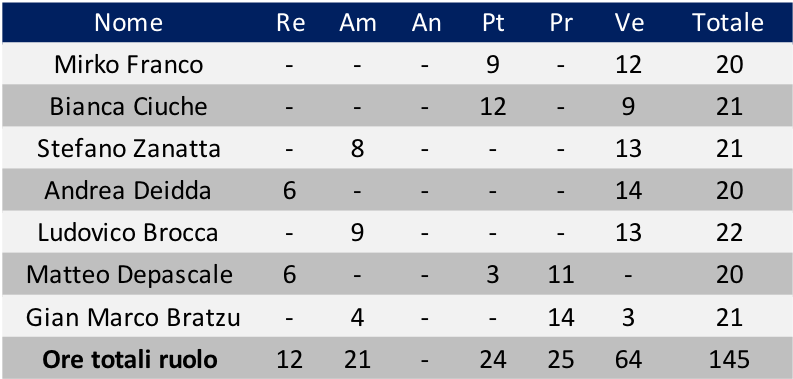
\includegraphics[scale=0.90]{images/tabellaValidazioneCollaudo.png}
		\end{tabular}
		\caption{Prospetto orario nel periodo di Validazione e Collaudo}
	\end{center}
\end{table}

Il seguente grafico mostra una rappresentazione visiva della suddivisione oraria dei ruoli all'interno del gruppo:
\begin{figure}[!ht]
	\begin{center}
		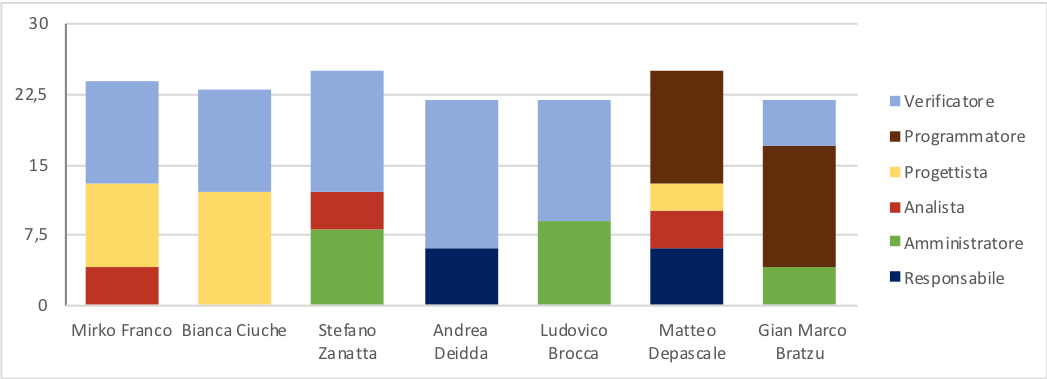
\includegraphics[scale=0.90]{images/grafoValidazioneCollaudo.png}
		\caption{Grafico prospetto orario nel periodo di Validazione e Collaudo}
	\end{center}
\end{figure}

\subsection{Prospetto economico}
Il prospetto economico durante il periodo di Validazione e Collaudo è illustrato nella seguente tabella:

\begin{table}[!ht]
	\begin{center}
		\begin{tabular}{c}
			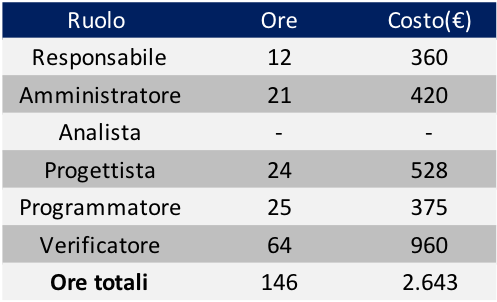
\includegraphics{images/tabellaValidazioneCollaudoEuro.png}
		\end{tabular}
		\caption{Prospetto Economico nel periodo di Validazione e Collaudo}
	\end{center}
\end{table}

La raffigurazione grafica del peso di ogni ruolo sul costo totale è così rappresentata:
\begin{figure}[!ht]
	\begin{center}
		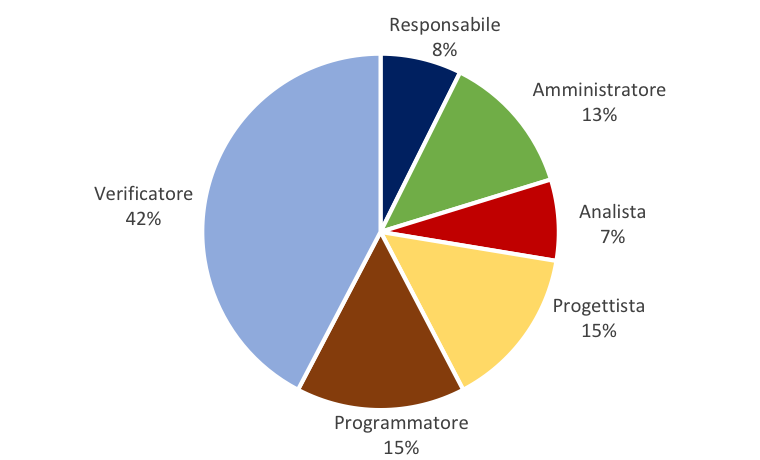
\includegraphics{images/grafoValidazioneCollaudoEuro.png}
		\caption{Grafico prospetto economico nel periodo di Validazione e Collaudo}
	\end{center}
\end{figure}
\newpage
\section{Totale ore rendicontate}
\subsection{Totale del  prospetto orario rendicontato}
Il totale del prospetto orario rendicontato è illustrato nella seguente tabella:

\begin{table}[!ht]
	\begin{center}
		\begin{tabular}{c}
			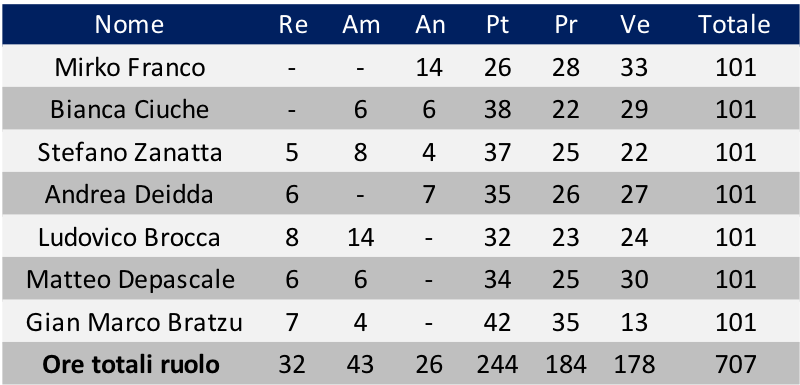
\includegraphics{images/tabellaOreRendicontate.png}
		\end{tabular}
		\caption{Prospetto orario totale delle ore rendicontate}
	\end{center}
\end{table}

Il seguente grafico mostra una rappresentazione visiva della suddivisione oraria dei ruoli all'interno del gruppo:
\begin{figure}[!ht]
	\begin{center}
		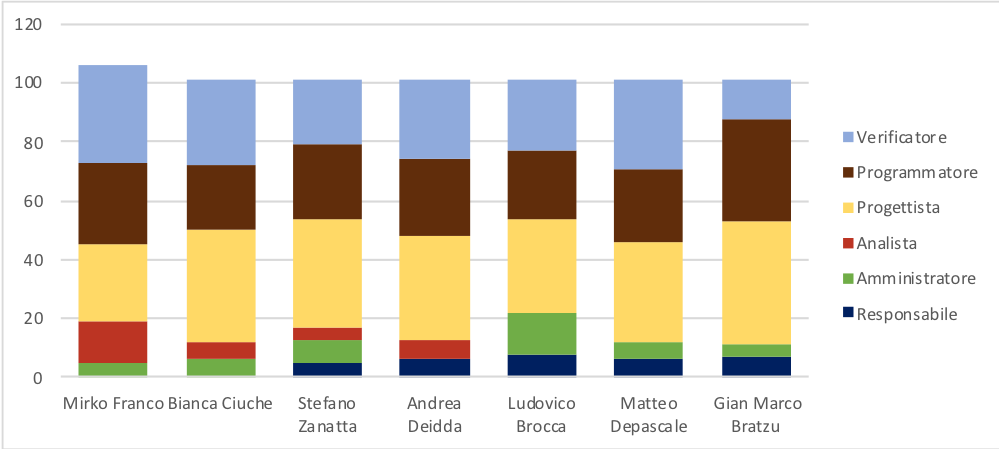
\includegraphics[scale=0.80]{images/grafoOreRendicontate.png}
		\caption{Grafico prospetto orario totale delle ore rendicontate}
	\end{center}
\end{figure}

\subsection{Totale del prospetto economico rendicontato}
Il totale del prospetto economico rendicontato che  include le ore rendicontate nel preventivo a carico del committente cioè dei periodi di Progettazione della Base Tecnologica, Progettazione di Dettaglio e Codifica e il periodo di Validazione e Collaudo è illustrato nella seguente tabella:

\begin{table}[!ht]
	\begin{center}
		\begin{tabular}{c}
			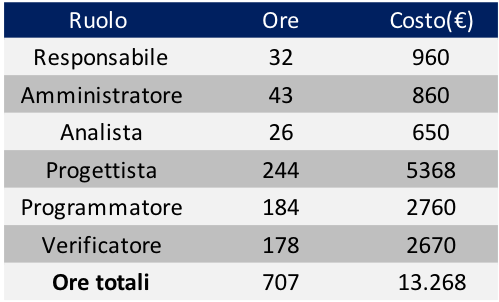
\includegraphics{images/tabellaOreRendicontateEuro.png}
		\end{tabular}
		\caption{Prospetto economico totale delle ore rendicontate}
	\end{center}
\end{table}

La raffigurazione grafica del peso di ogni ruolo sul costo totale è così rappresentata:

\begin{figure}[!ht]
	\begin{center}
		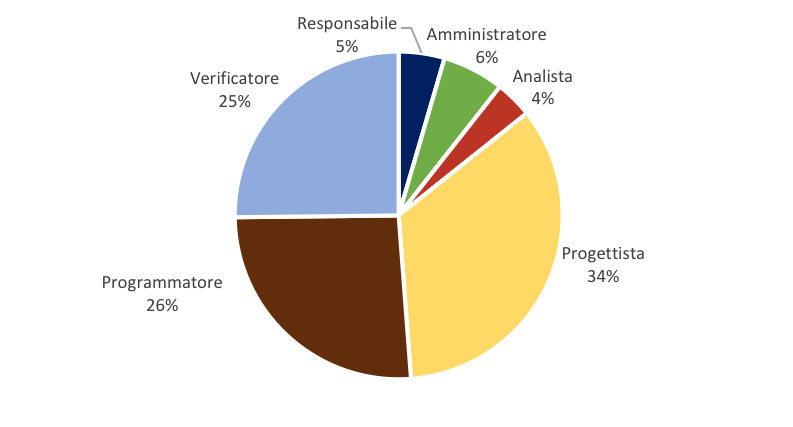
\includegraphics[scale=0.90]{images/grafoOreRendicontateEuro.png}
		\caption{Grafico prospetto economico totale delle ore rendicontate}
	\end{center}
\end{figure}

\section{Totale ore con investimento}
\subsection{Totale del prospetto orario con investimento}
Il totale del prospetto orario con investimento che include sia le ore rendicontate nel preventivo a carico del committente sia le ore di investimento iniziali,è illustrato nella seguente tabella:

\begin{table}[!ht]
	\begin{center}
		\begin{tabular}{c}
			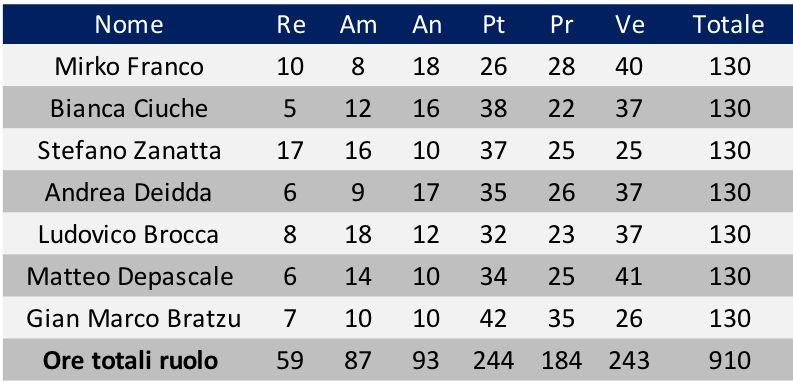
\includegraphics[scale=0.80]{images/tabellaOreInvestimento.png}
		\end{tabular}
		\caption{Prospetto orario totale delle ore di investimento e rendicontate}
	\end{center}
\end{table}

Il seguente grafico mostra una rappresentazione visiva della suddivisione oraria dei ruoli all'interno del gruppo:
\begin{figure}[!ht]
	\begin{center}
		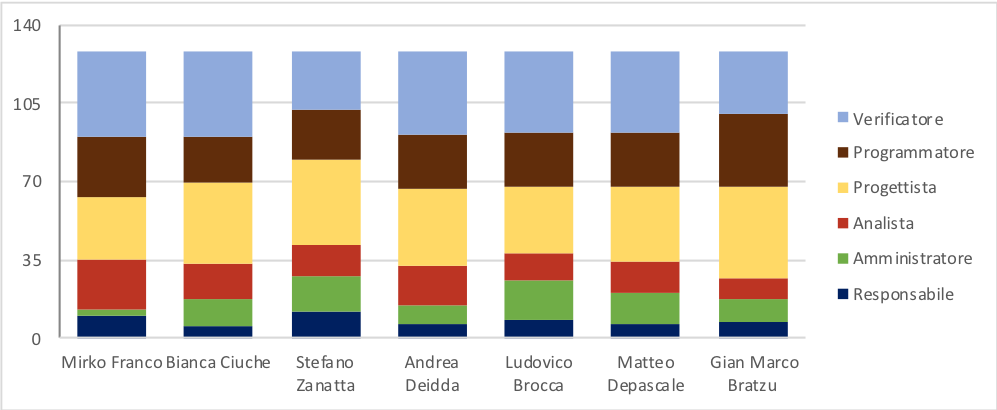
\includegraphics[scale=0.80]{images/grafoOreInvestimento.png}
		\caption{Grafico prospetto orario totale delle ore di investimento e rendicontate}
	\end{center}
\end{figure}

\subsection{Totale del prospetto economico con investimento}
Il totale del prospetto economico con investimento che include sia le ore rendicontate nel preventivo a carico del committente sia  le ore  di investimento iniziali per l'intera durata del progetto è illustrato nella seguente tabella:
\begin{table}[!ht]
	\begin{center}
		\begin{tabular}{c}
			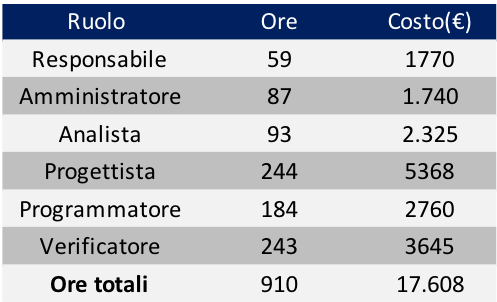
\includegraphics{images/tabellaOreInvestimentoEuro.png}
		\end{tabular}
		\caption{Prospetto economico totale delle ore di investimento e rendicontate}
	\end{center}
\end{table}

La raffigurazione grafica del peso di ogni ruolo sul costo totale è così rappresentata:
\begin{figure}[!ht]
	\begin{center}
		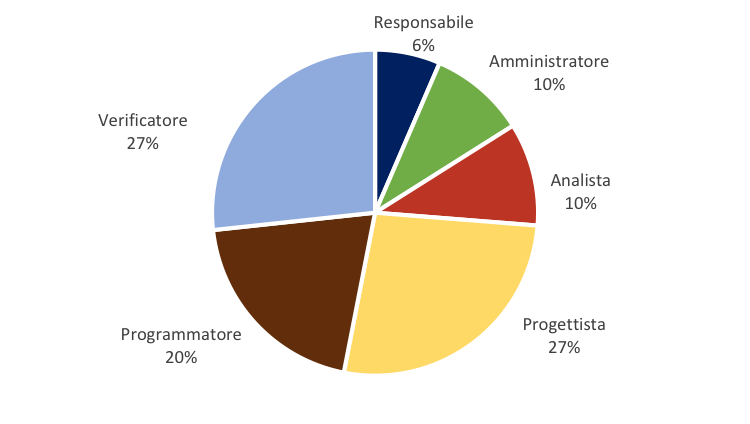
\includegraphics{images/grafoOreInvestimentoEuro.png}
		\caption{Grafico prospetto economico totale delle ore di investimento e rendicontate}
	\end{center}
\end{figure}



